\begin{flushleft}
\section{Bellmanvisor}
{\Large Carl Michael Bellman (1740-1795) hör till de största svenska skalderna.
Han levde ett glatt liv i Stockholm och sågs ofta på societetskrogen Den Gyllene Freden, liksom på sjaskiga hak på Södermalm.
I dessa miljöer fann Bellman sin inspiration till visornas mustiga karaktärer - Movitz, Fredman, Ulla Winblad...
Vi gillar Bellman och har därför givit hans visor ett eget kapitel i Encyclopedia Gasquica.}
\end{flushleft}

\vspace{2cm}
\begin{center}
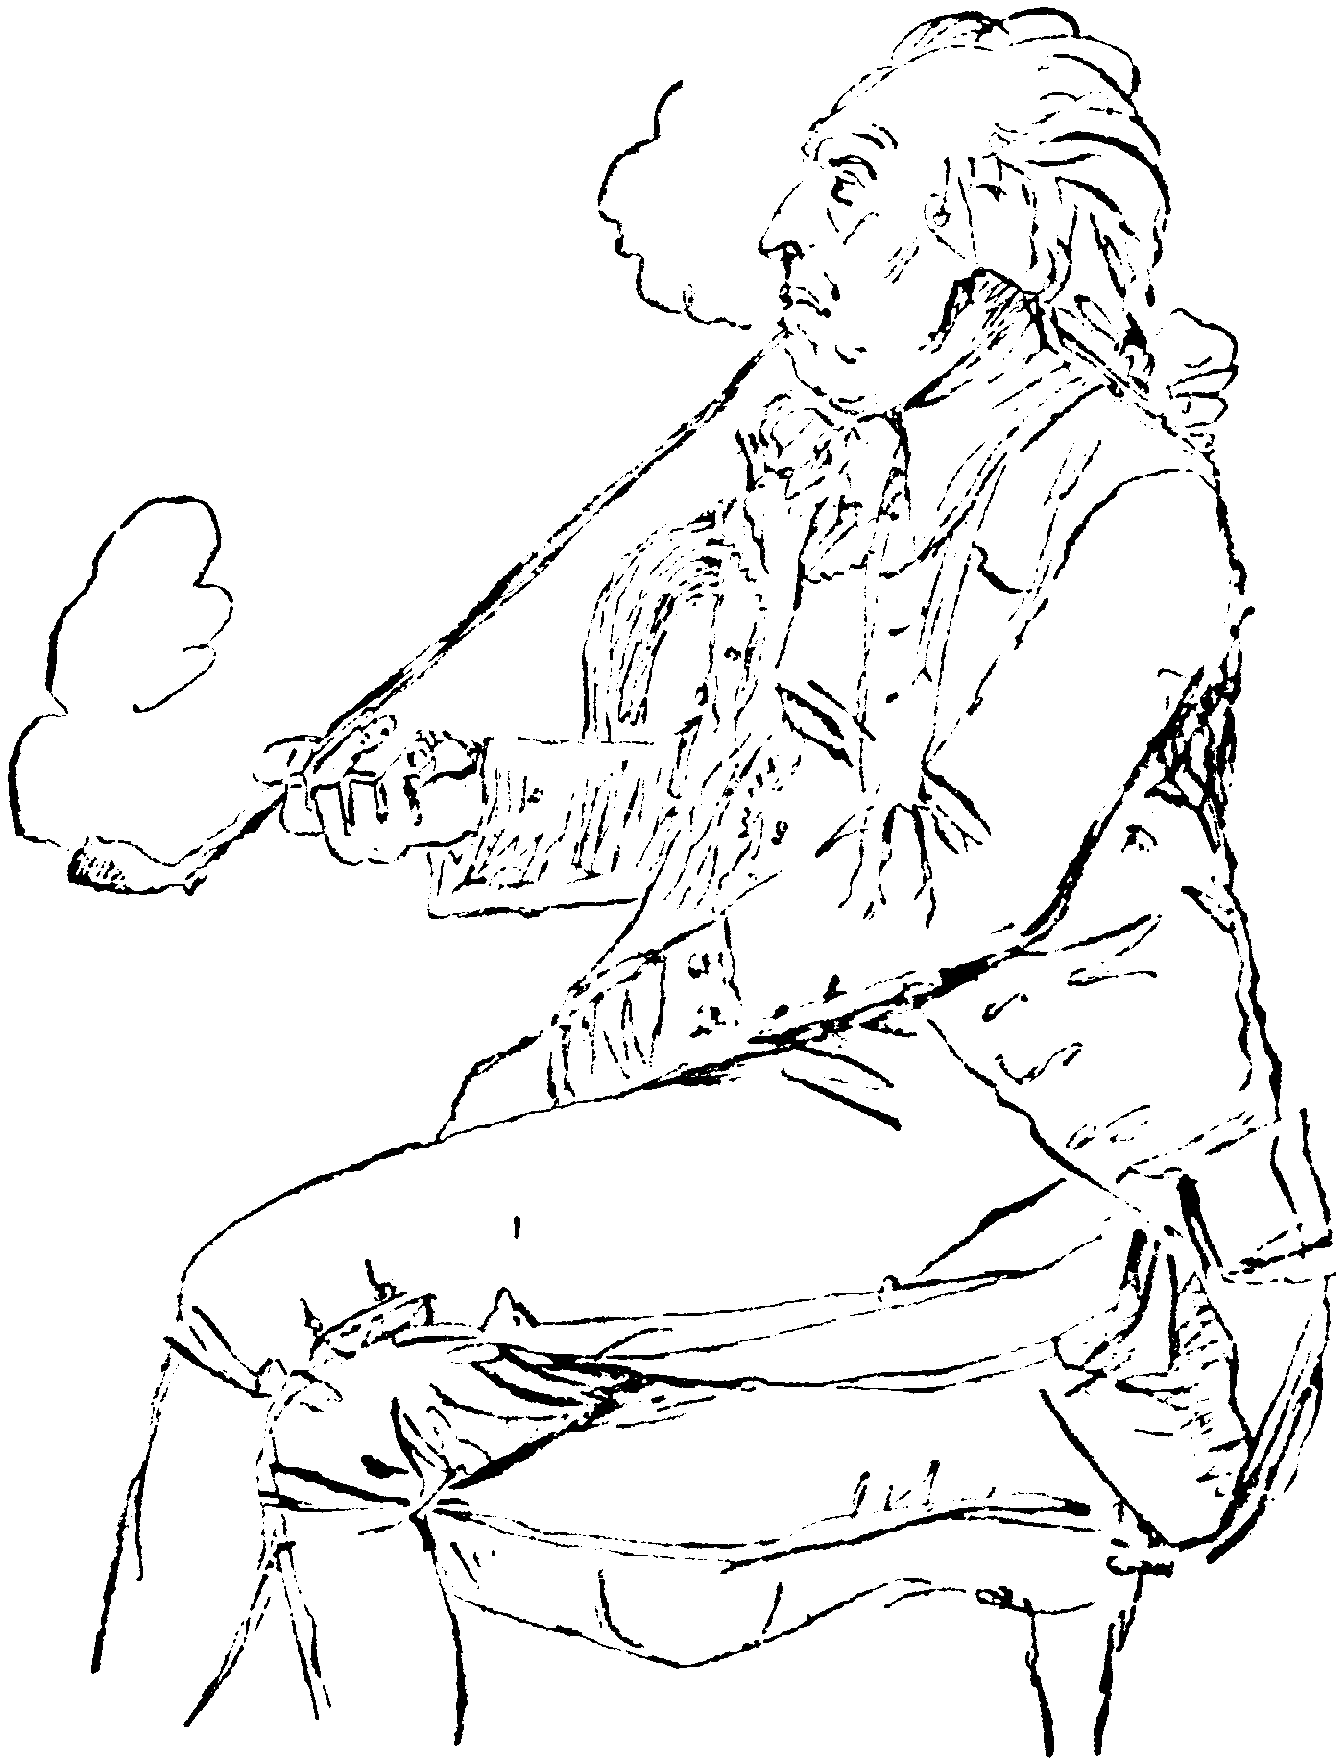
\includegraphics[width=6cm]{bilder/bellman.png}
\end{center}
\newpage

\inputsong{fredmanssangno35}
\inputsong{fjarilnvingad}
\inputsong{fredmanssangno21}
\newpage
\inputsong{epistel81}
\newpage
\inputsong{epistel01}
\newpage
\inputsong{solenglimmar}
\kom{(Då orginalsången har 21 verser valde\\
vi att ta med den första och sista)}
%Liksom en herdinna
